\documentclass{beamer}
 
\usepackage[utf8]{inputenc}
\usepackage[english]{babel}
\usepackage{amsmath}
\usepackage{amsfonts}
\usepackage{amssymb}
\usepackage{graphicx} 
\usepackage{latexsym} 
\usepackage{listings}
\usepackage{xcolor}
\usepackage{soul}
\usepackage[T1]{fontenc}
\usepackage{amsthm}
\usepackage{mathtools}
\usepackage{setspace}
\usepackage{array,multirow,makecell}
\usepackage{geometry}
\usepackage{textcomp}
\usepackage{float}
\usepackage{bbold}
\usepackage{wrapfig}
\usepackage{textpos}

\rmfamily

\usetheme{Madrid}
%%\usecolortheme{beaver}



\title{Gaz réels, gaz parfait}
\author{Naïmo Davier}
\institute{Université Paul sabatier}
\date{Agrégation 2019}

 
\begin{document}
	
\begin{frame}
	\titlepage
\end{frame}

\addtocounter{framenumber}{-1}

%\begin{frame}
%\frametitle{Lois empiriques pour le gaz parfait}
%\begin{itemize}
%	\item Loi de Boyle et Mariotte :\\
%	"A température constante le produit de la pression par le volume PV est constant".
%	\item Loi d'Avogadro :\\
%	"Des volumes égaux de gaz parfaits, à la même pression et à la même température contiennent le même nombre de moles".
%	\item Loi de Gay Lussac :\\
%	"A pression constante le volume occupé par une quantité déterminée de gaz est proportionnel à la température T".
%	\item Loi de J.Charles :\\
%	"A volume constant la pression d'une quantité déterminée de gaz parfait est proportionnelle à la température T".
%	\item Loi de J.Dalton :\\
%	"La pression d'un mélange de deux gaz est la somme des pression partielles".
%\end{itemize}
%\end{frame}
\begin{frame}
\frametitle{Gaz réels : un comportement commun à basse pression}
\centerline{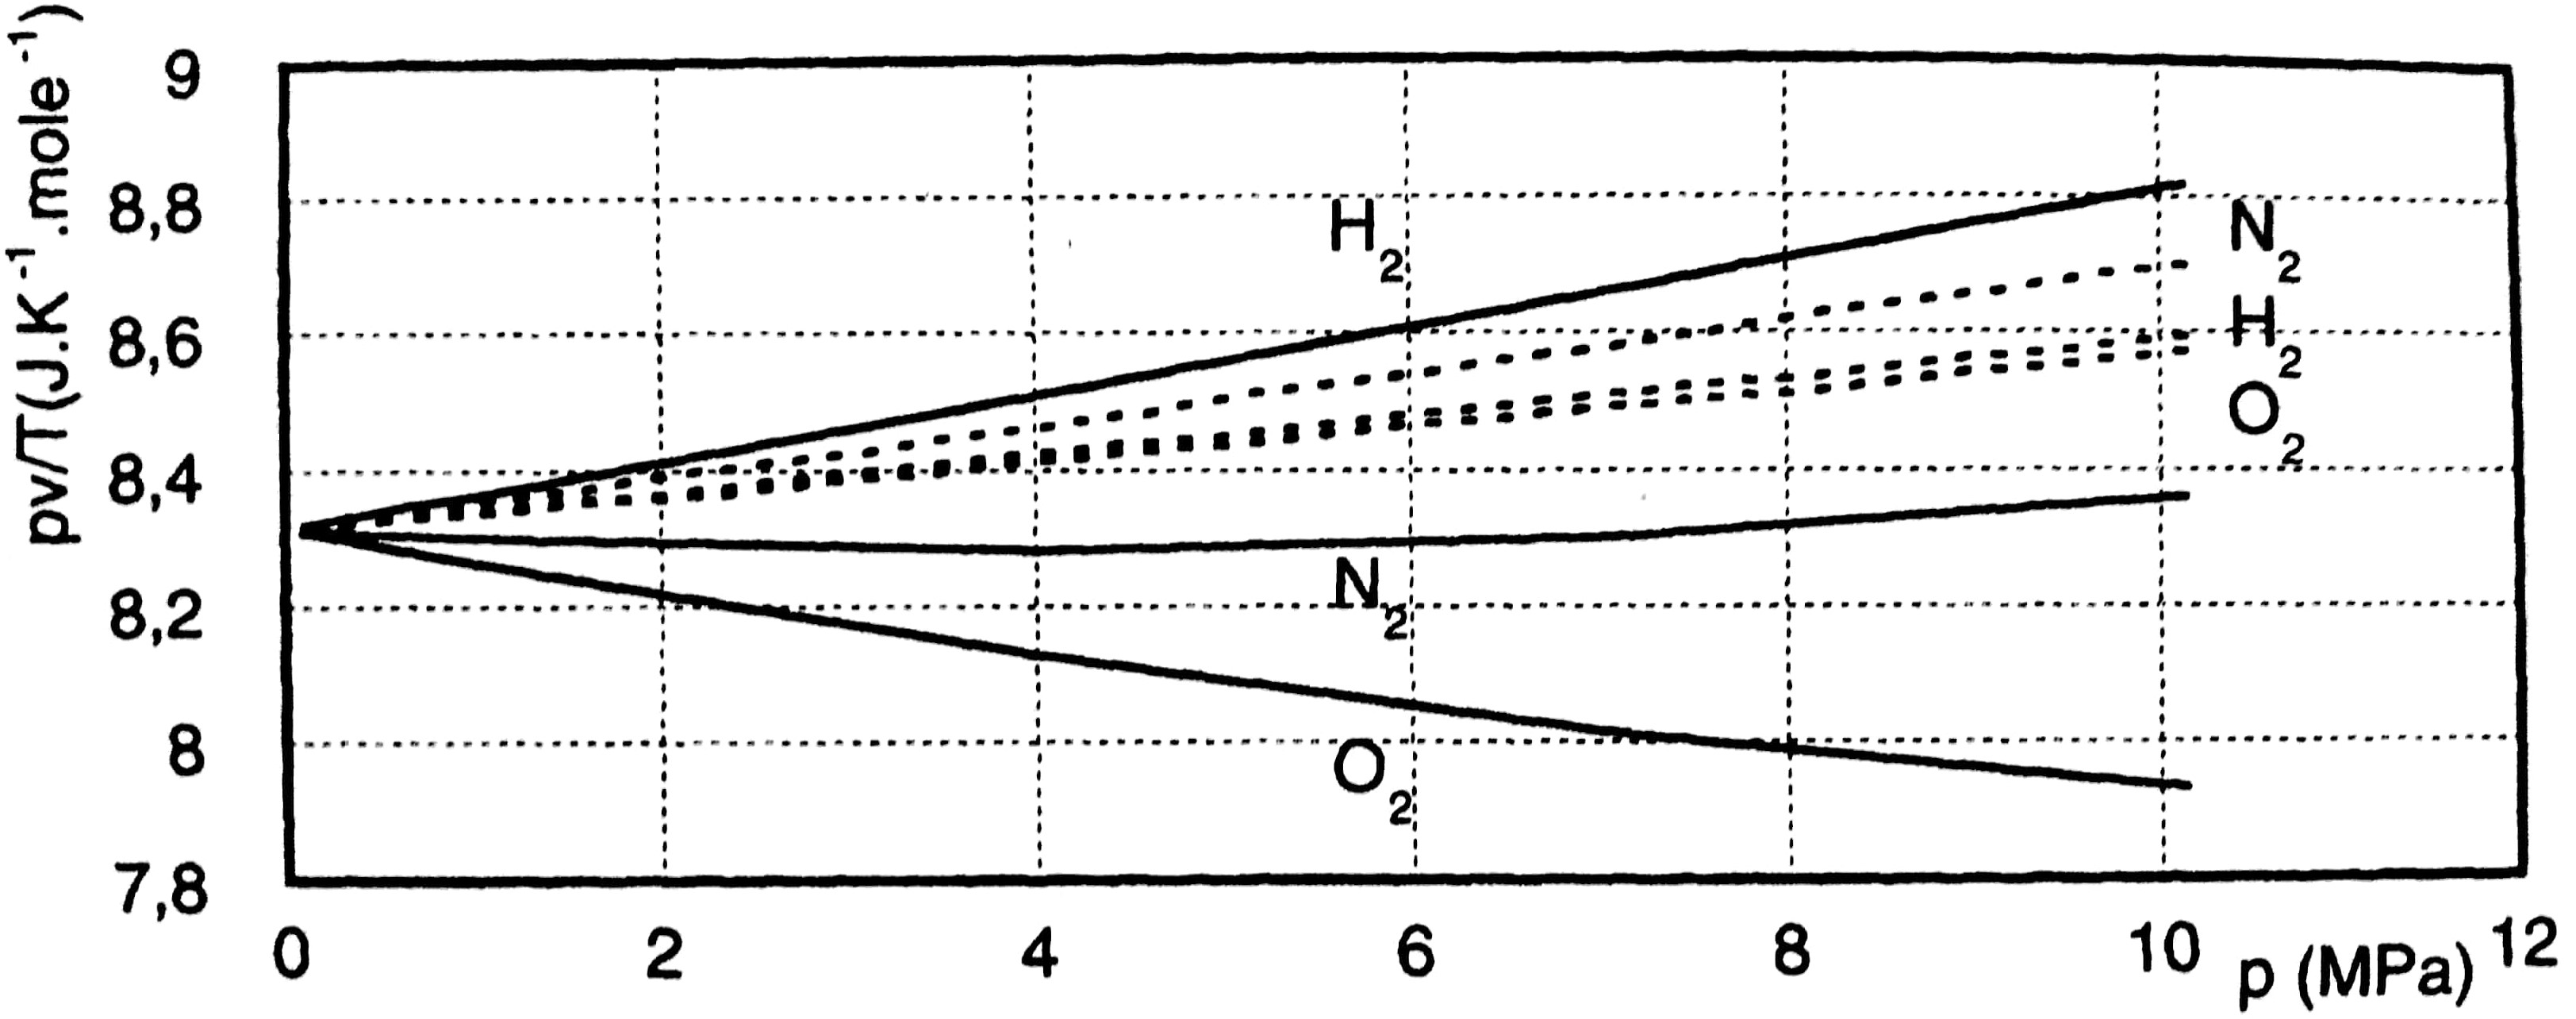
\includegraphics[width=11cm]{comportement_gaz_reels}}
\vspace{0.5cm}
traits pleins : $T = 300$ K, traits pointillés : $T=600$K
\end{frame}

\begin{frame}
\frametitle{Notion de pression}
\centerline{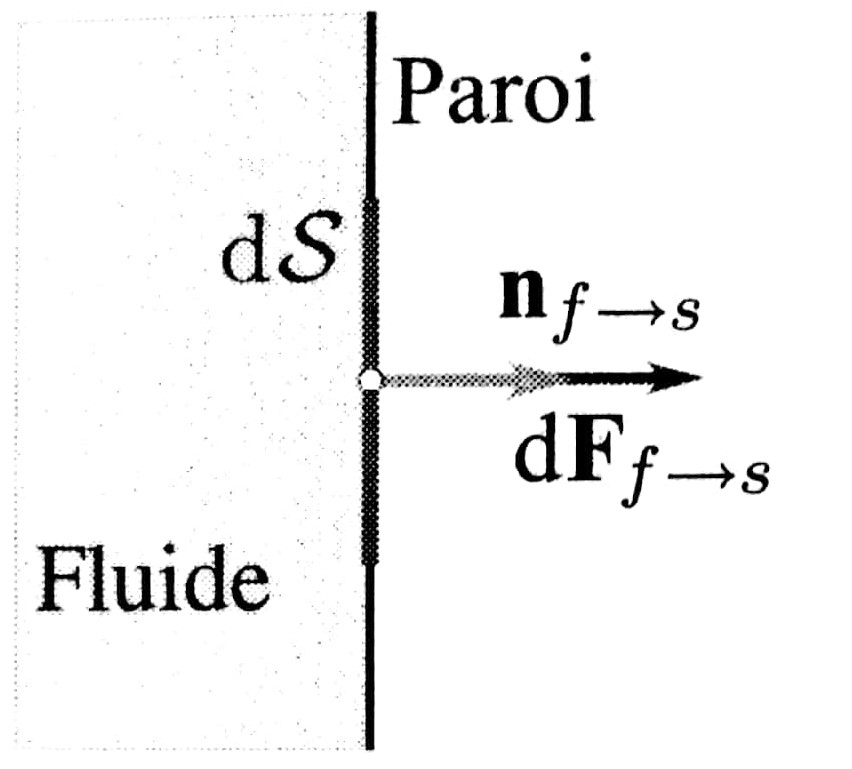
\includegraphics[width=5cm]{defP}}
\end{frame}

\begin{frame}
\frametitle{Calcul de la pression}
\centering 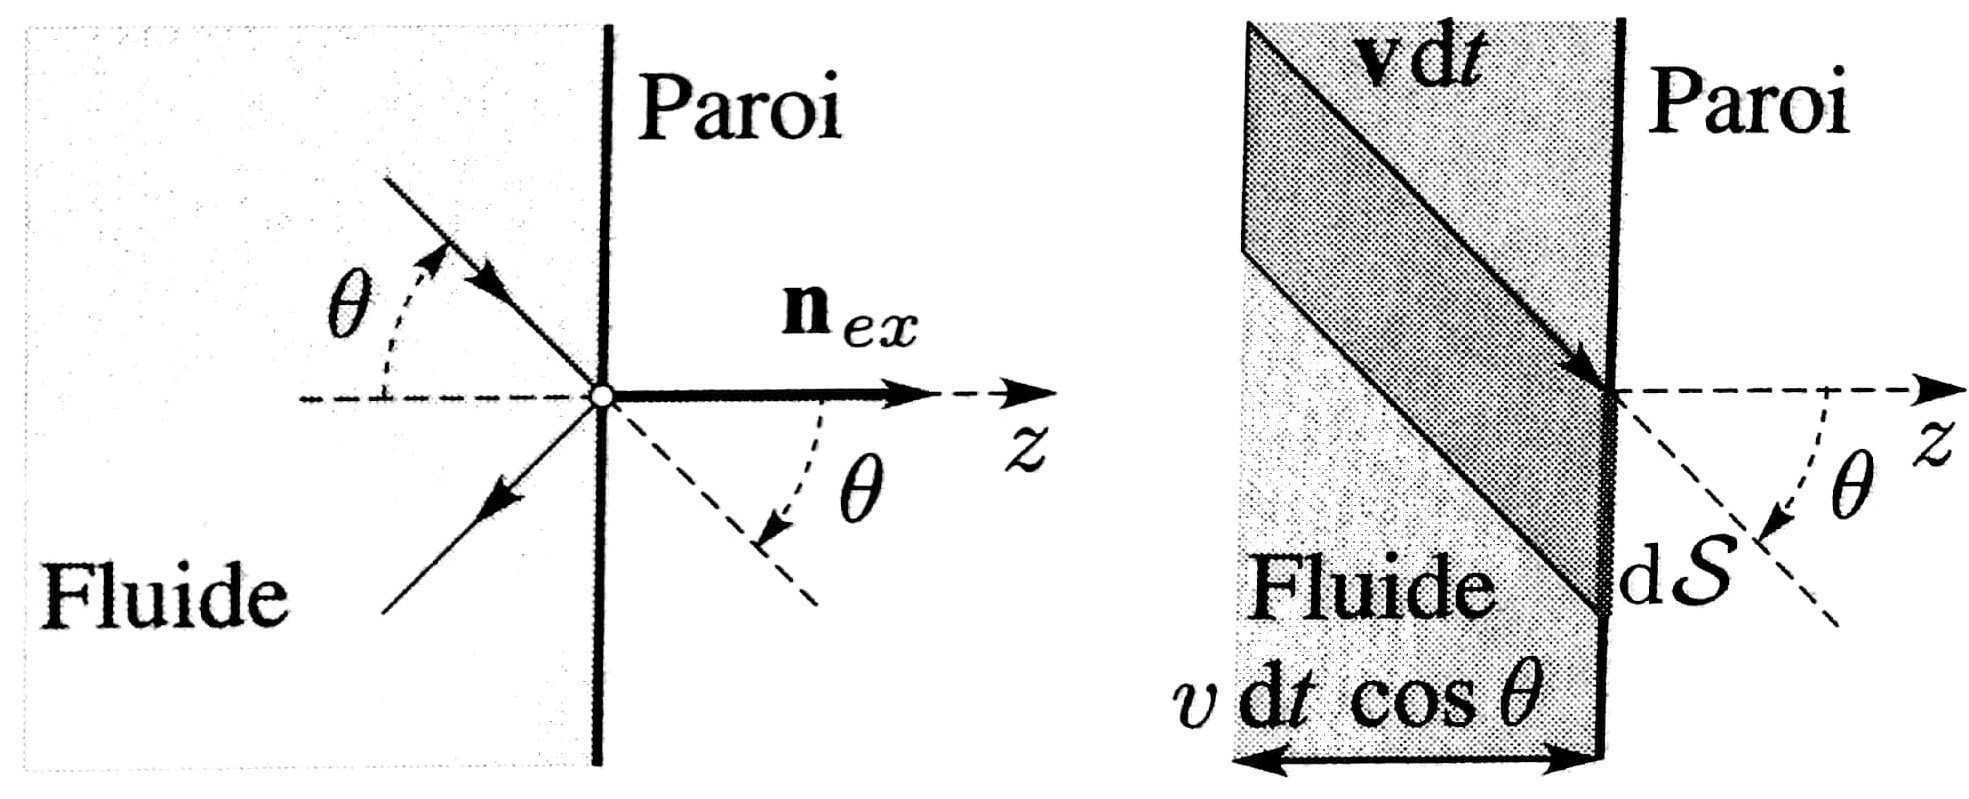
\includegraphics[width=10cm]{calcP}
\end{frame}

%\begin{frame}
%\frametitle{Lois empiriques et équation d'état : $PV=nRT$}
%\begin{itemize}
%	\item Loi de Boyle et Mariotte :\\
%	"A température constante le produit de la pression par le volume PV est constant" $\rightarrow PV=nRT$.
%	\item Loi d'Avogadro :\\
%	"Des volumes égaux de gaz parfaits, à la même pression et à la même température contiennent le même nombre de moles" $\rightarrow n=\frac{RT}{PV}$.
%	\item Loi de Gay Lussac :\\
%	"A pression constante le volume occupé par une quantité déterminée de gaz est proportionnel à la température T" $\rightarrow V=\frac{nR}{P}T$.
%	\item Loi de J.Charles :\\
%	"A volume constant la pression d'une quantité déterminée de gaz parfait est proportionnelle à la température T" $\rightarrow P=\frac{nR}{V}T$.
%	\item Loi de J.Dalton :\\
%	"La pression d'un mélange de deux gaz est la somme des pression partielles".
%\end{itemize}
%\end{frame}


\begin{frame}
\frametitle{Capacité calorifique}
\centerline{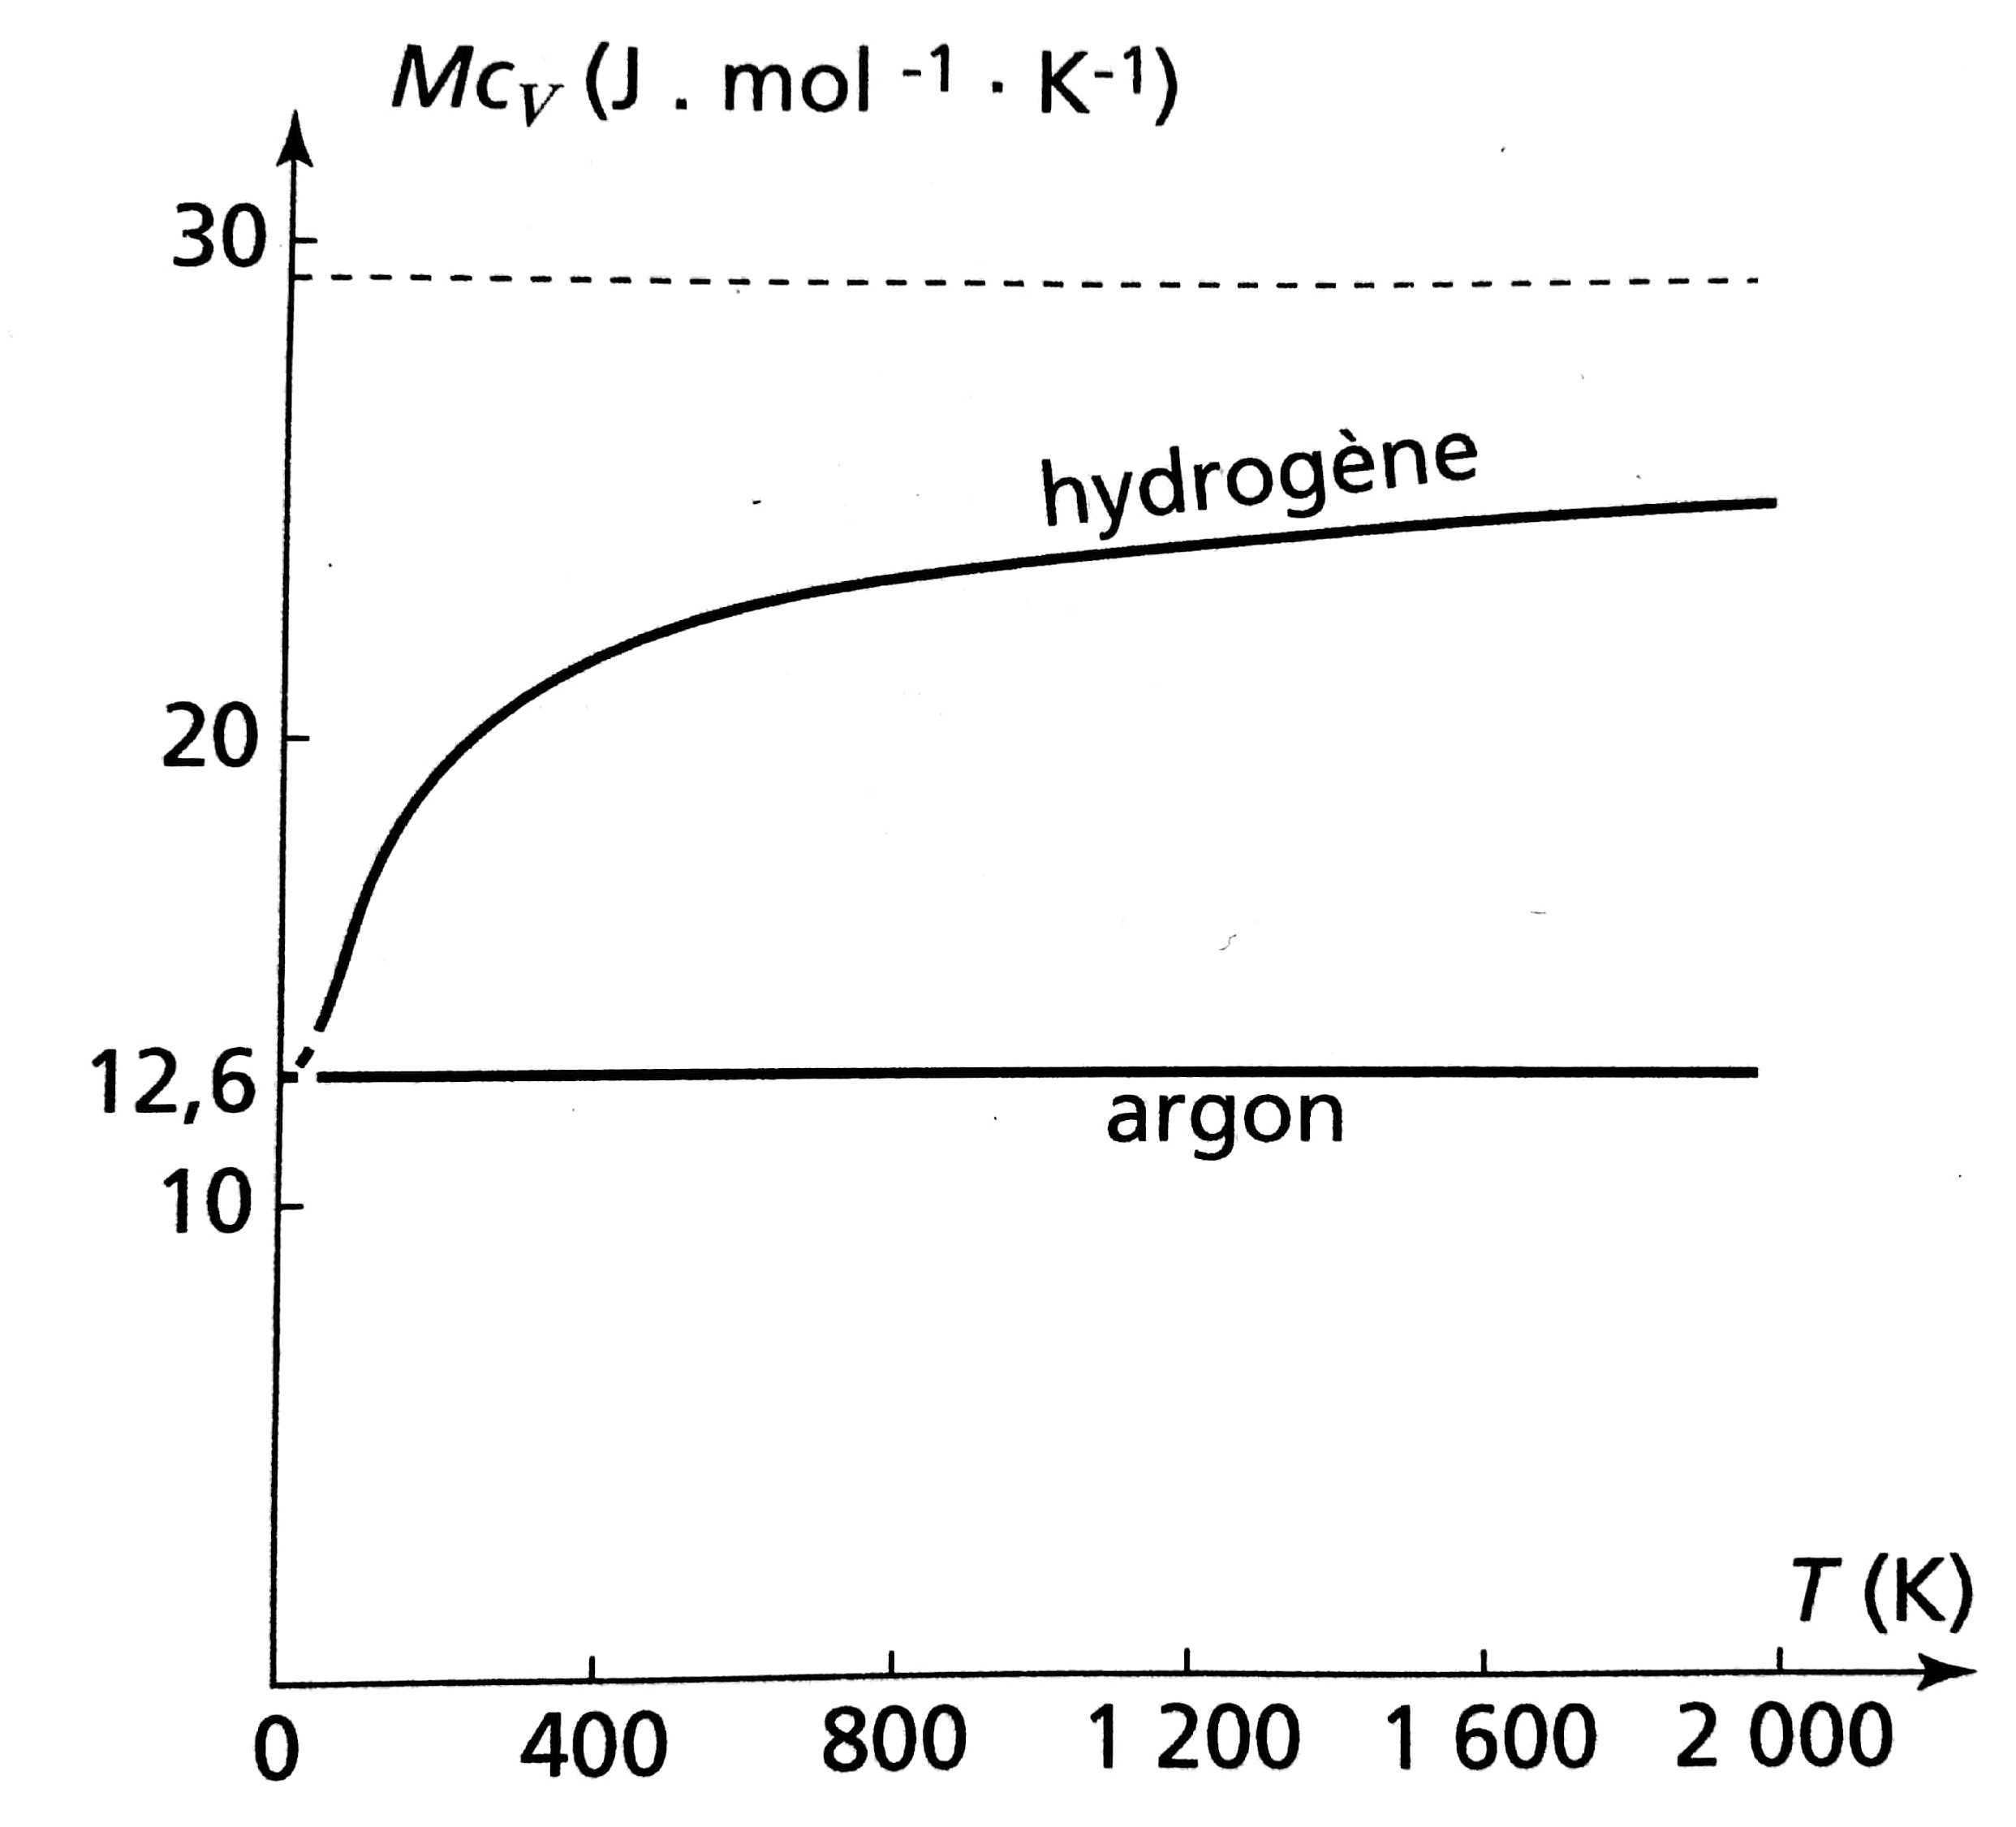
\includegraphics[width=8cm]{Cv}}
\end{frame}

\begin{frame}
\frametitle{Gel des degrés de liberté : températures caractéristiques}
\centerline{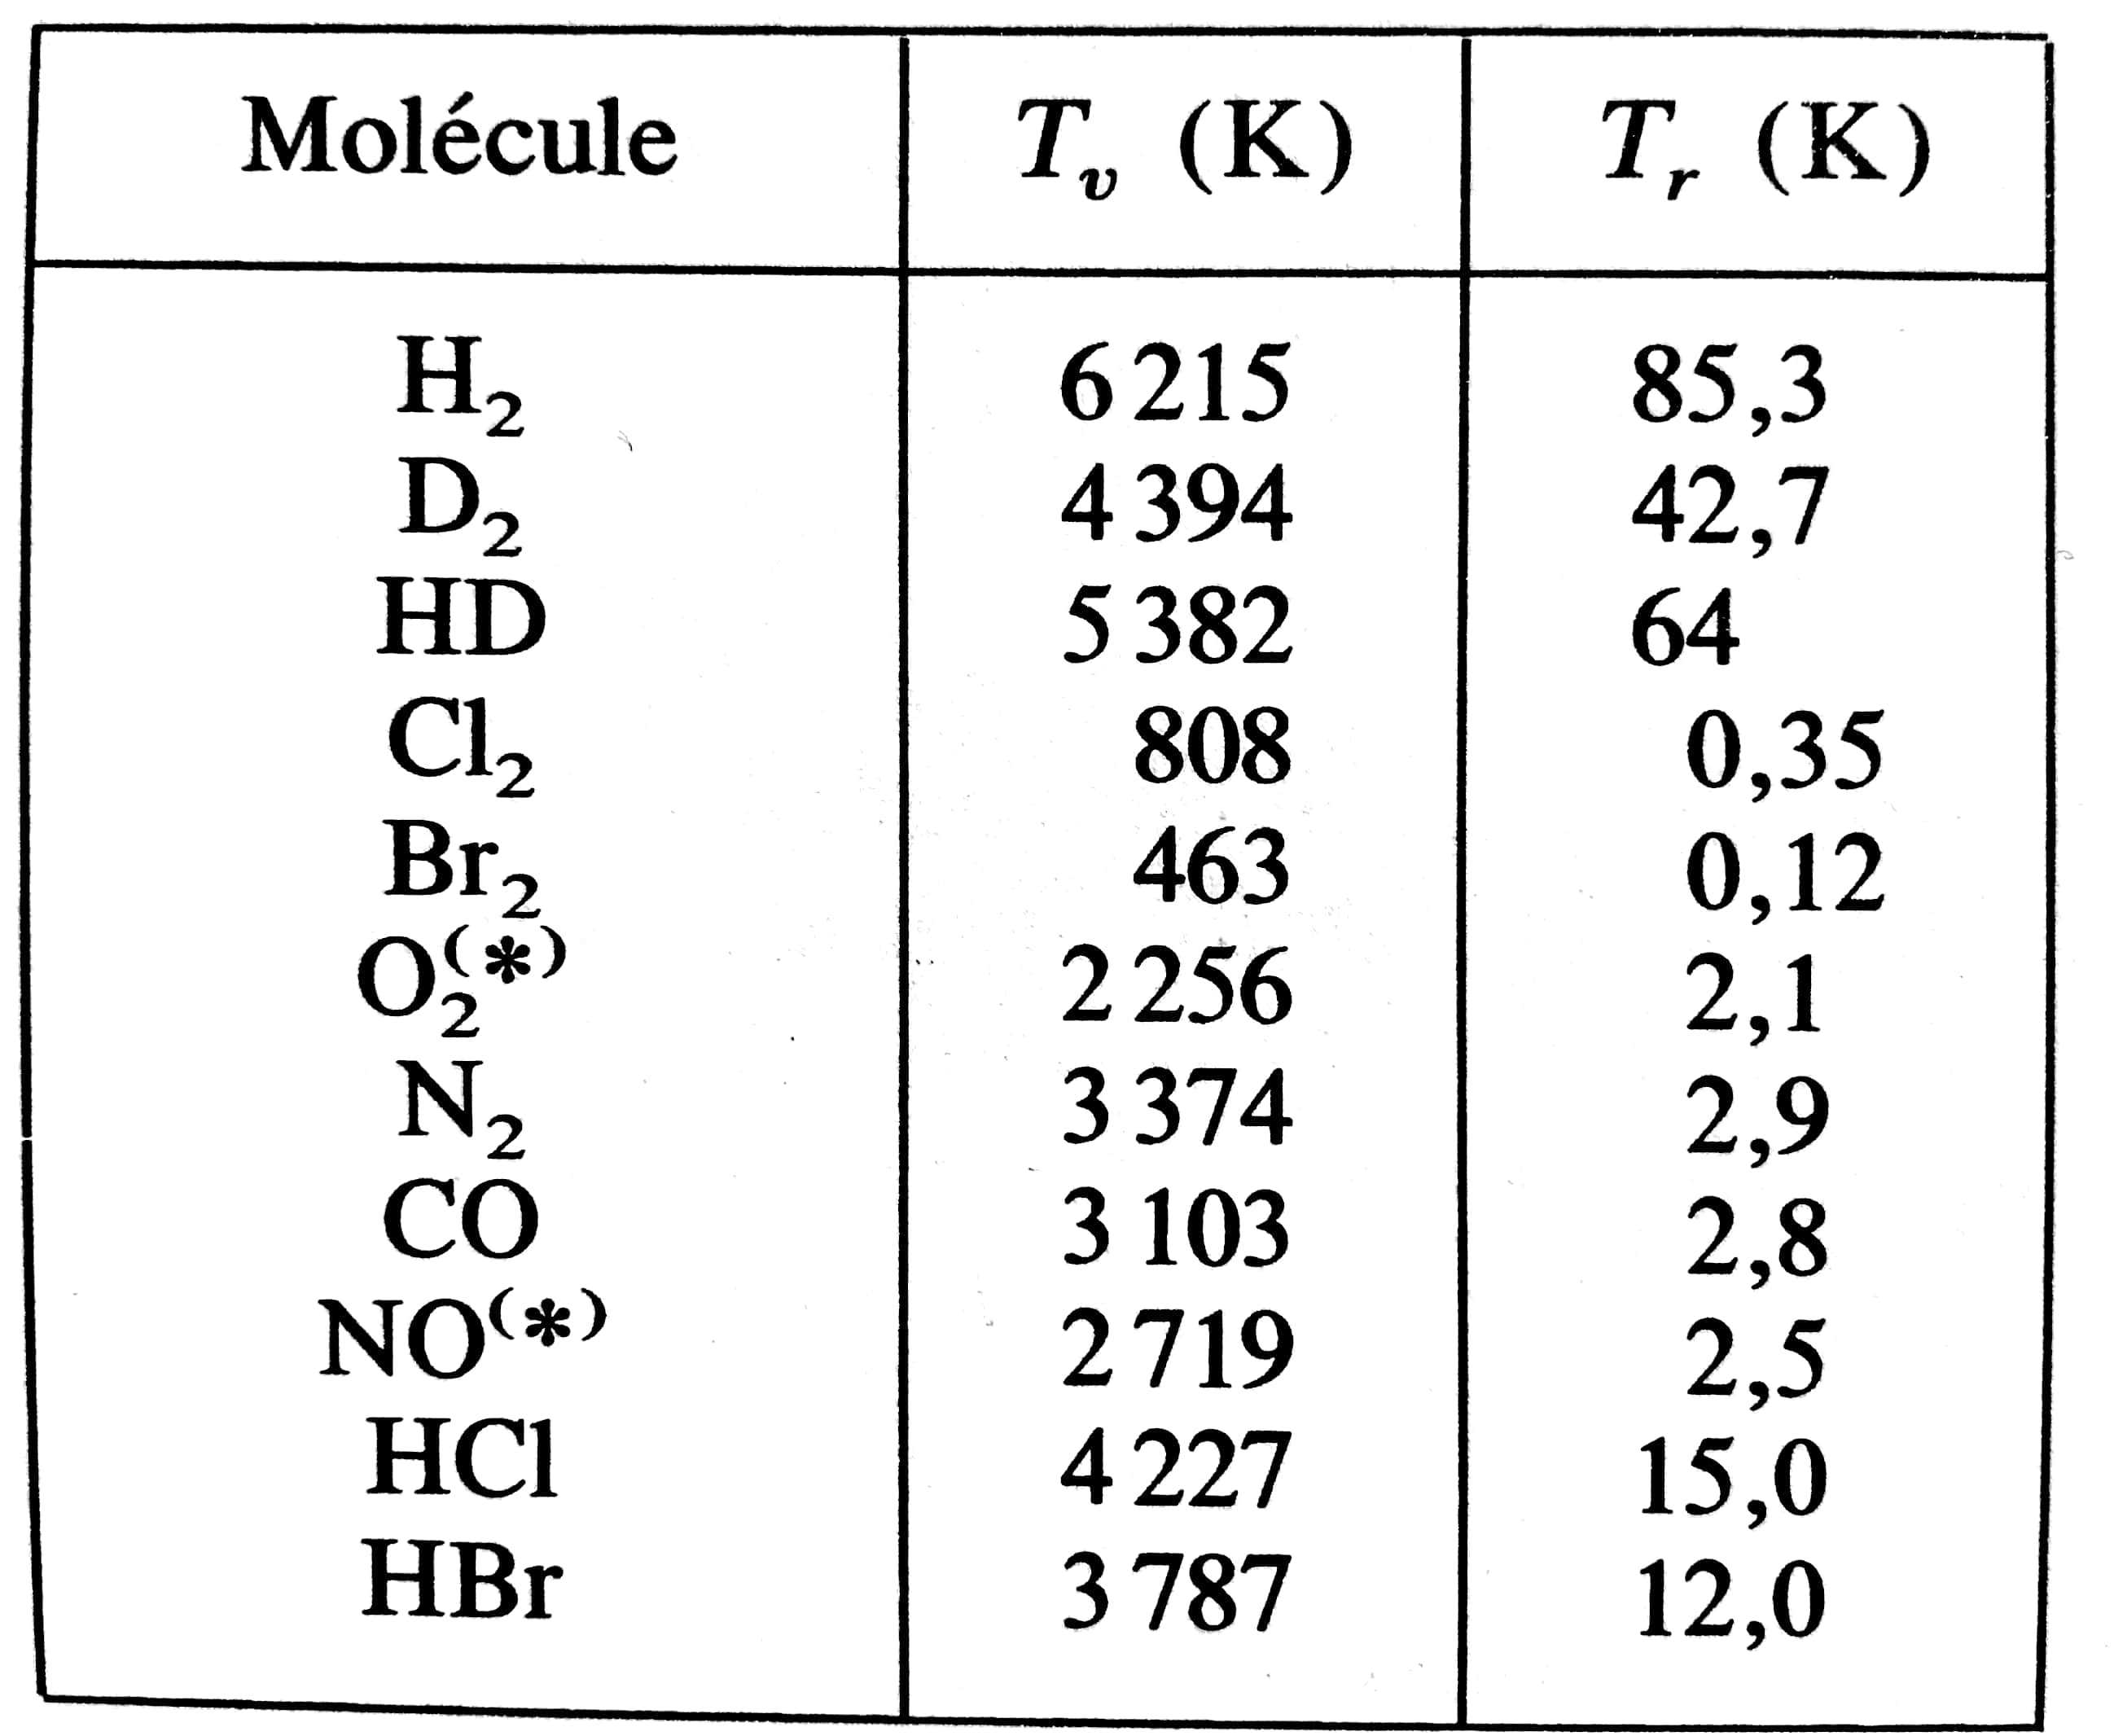
\includegraphics[width=8cm]{Tcaract}}
\end{frame}

\begin{frame}
\frametitle{Gaz de Van der Waals : potentiel d'interaction électrostatique}
\centerline {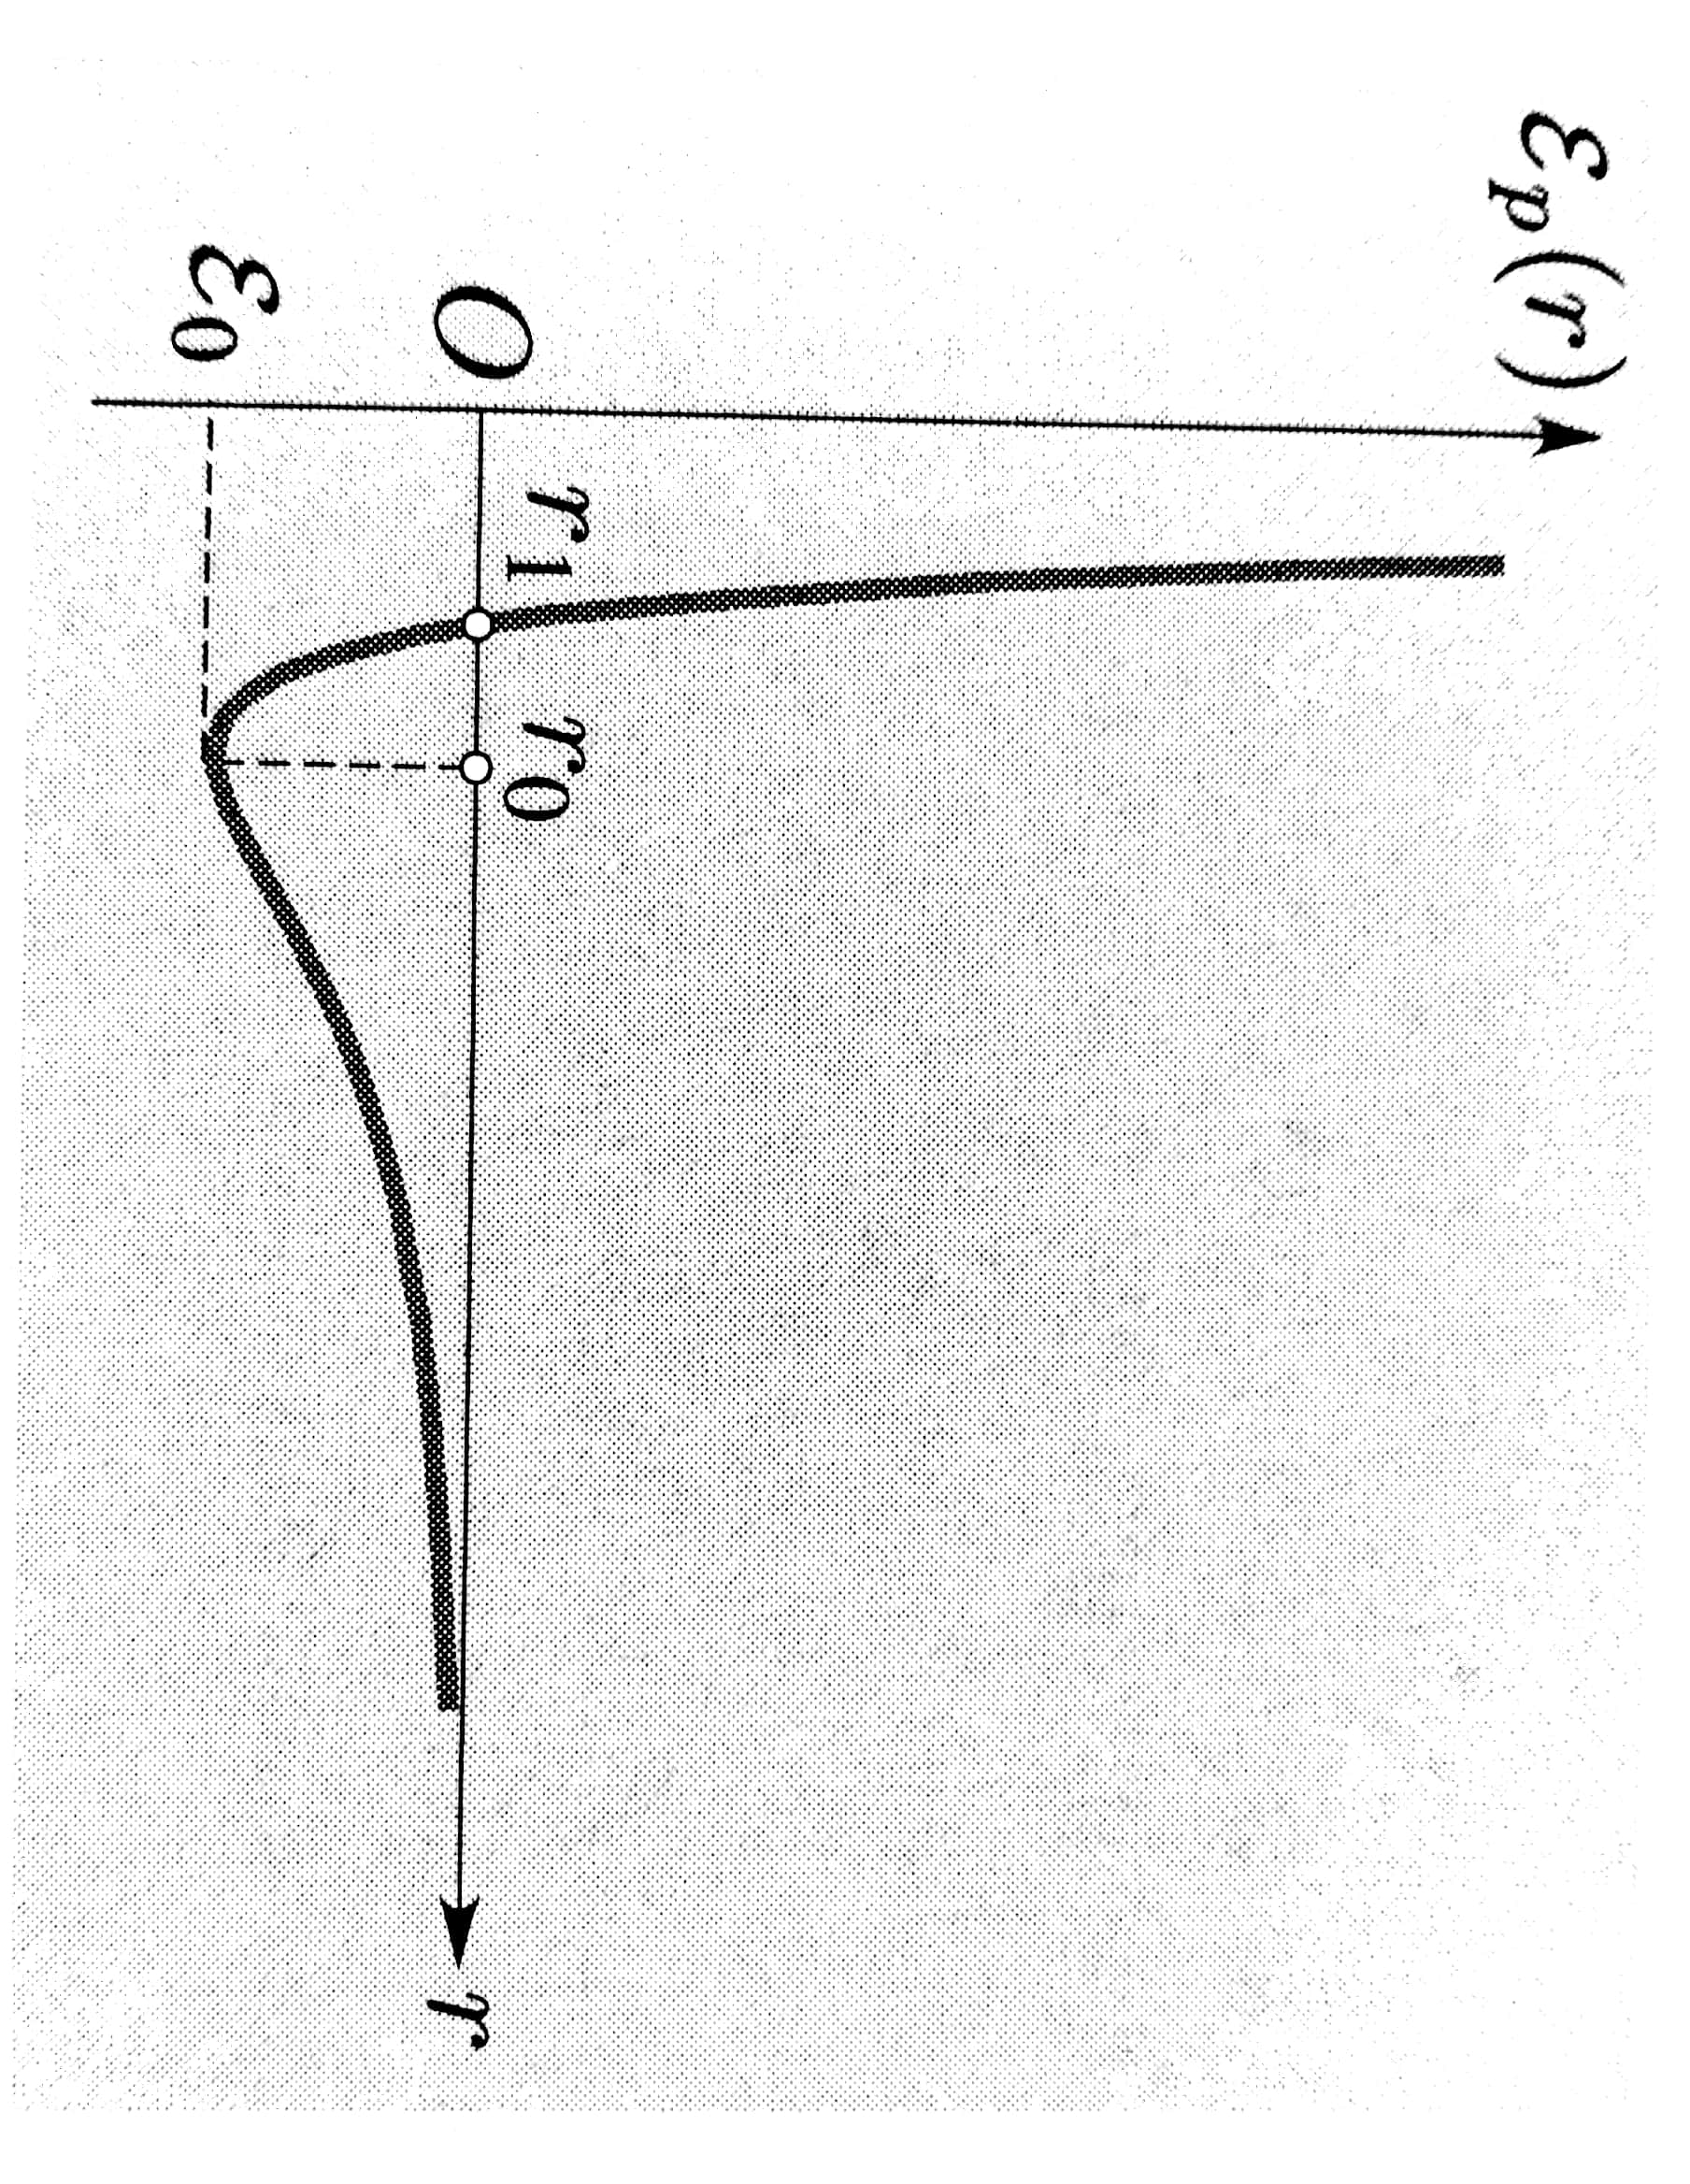
\includegraphics[width=6.5cm, angle=90]{VdW} }
\end{frame}

\begin{frame}
\frametitle{Gaz de Van der Waals : pression interne}
\centerline {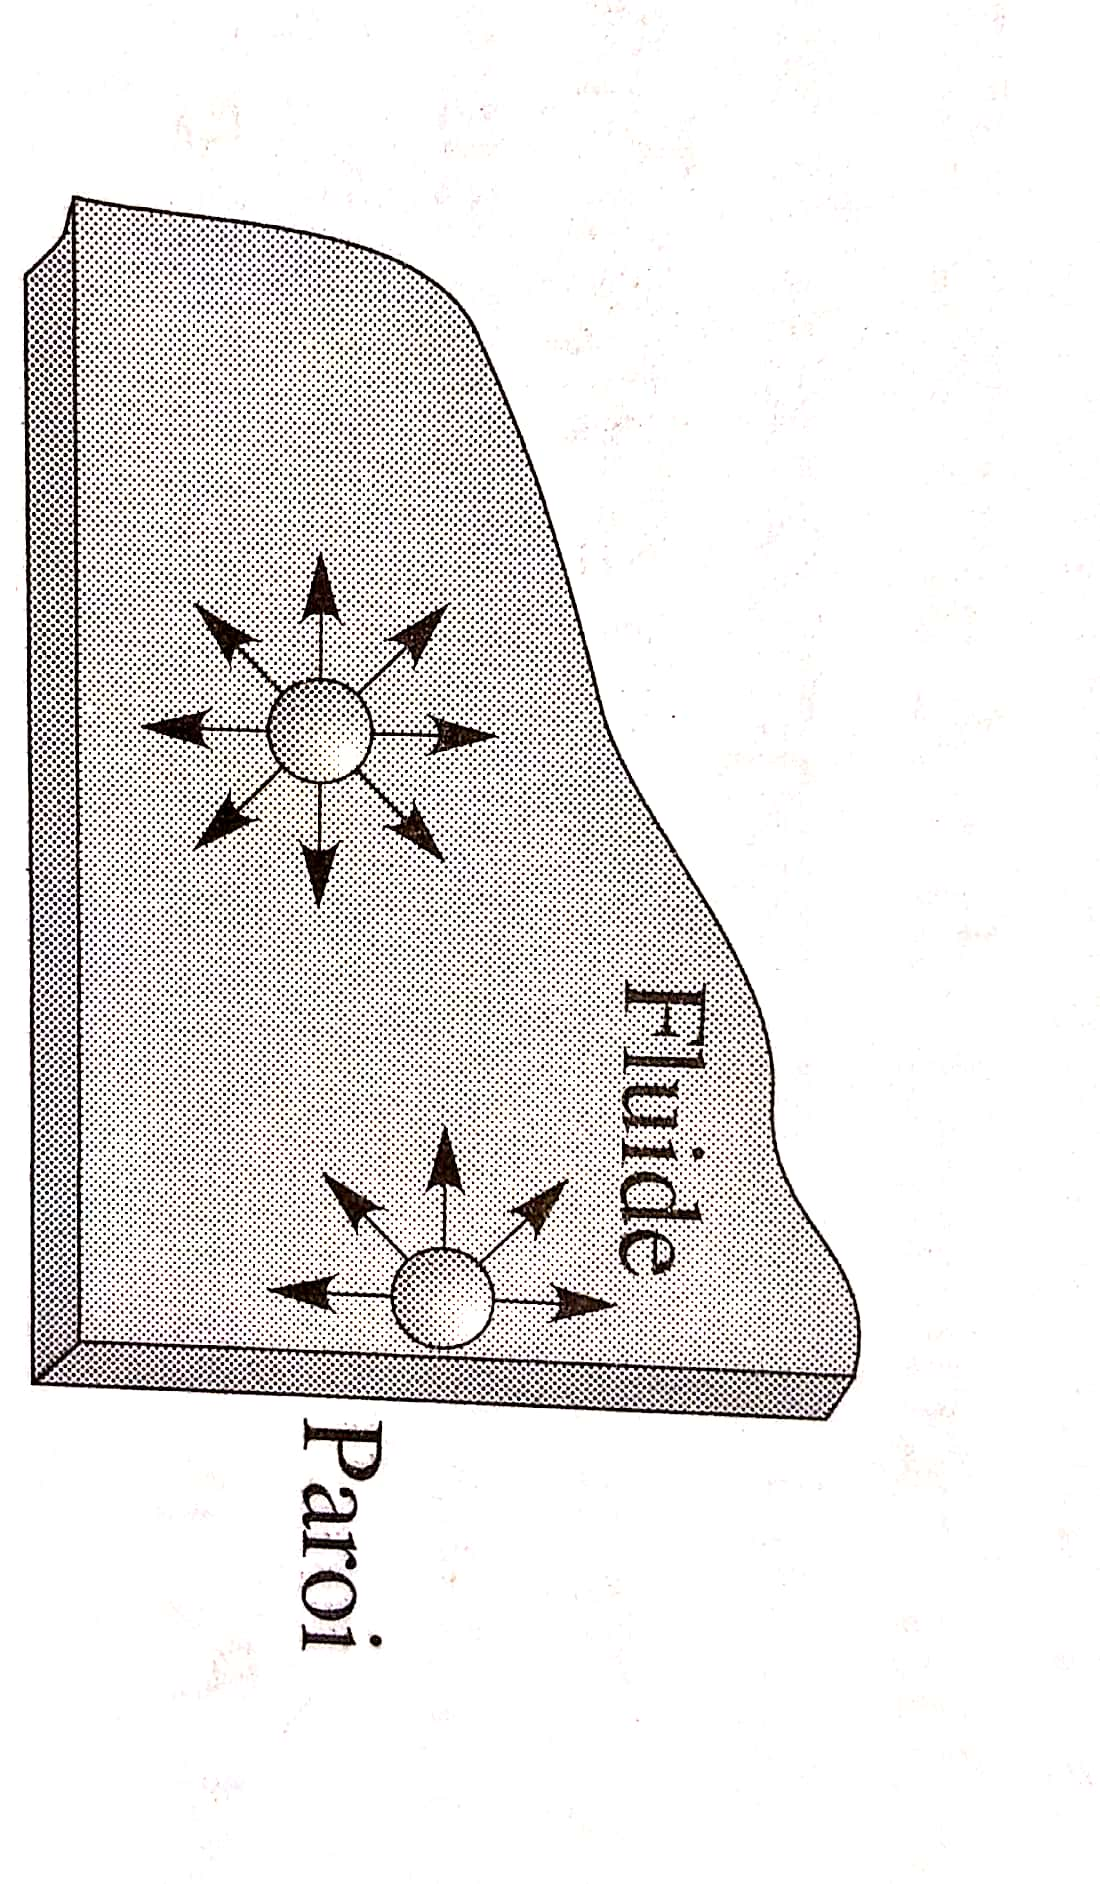
\includegraphics[width=5cm, angle=90]{Pint} }
\end{frame}


\end{document}